\documentclass[tikz,border=6pt]{standalone}
\usetikzlibrary{positioning, arrows.meta, fit, calc}

\begin{document}
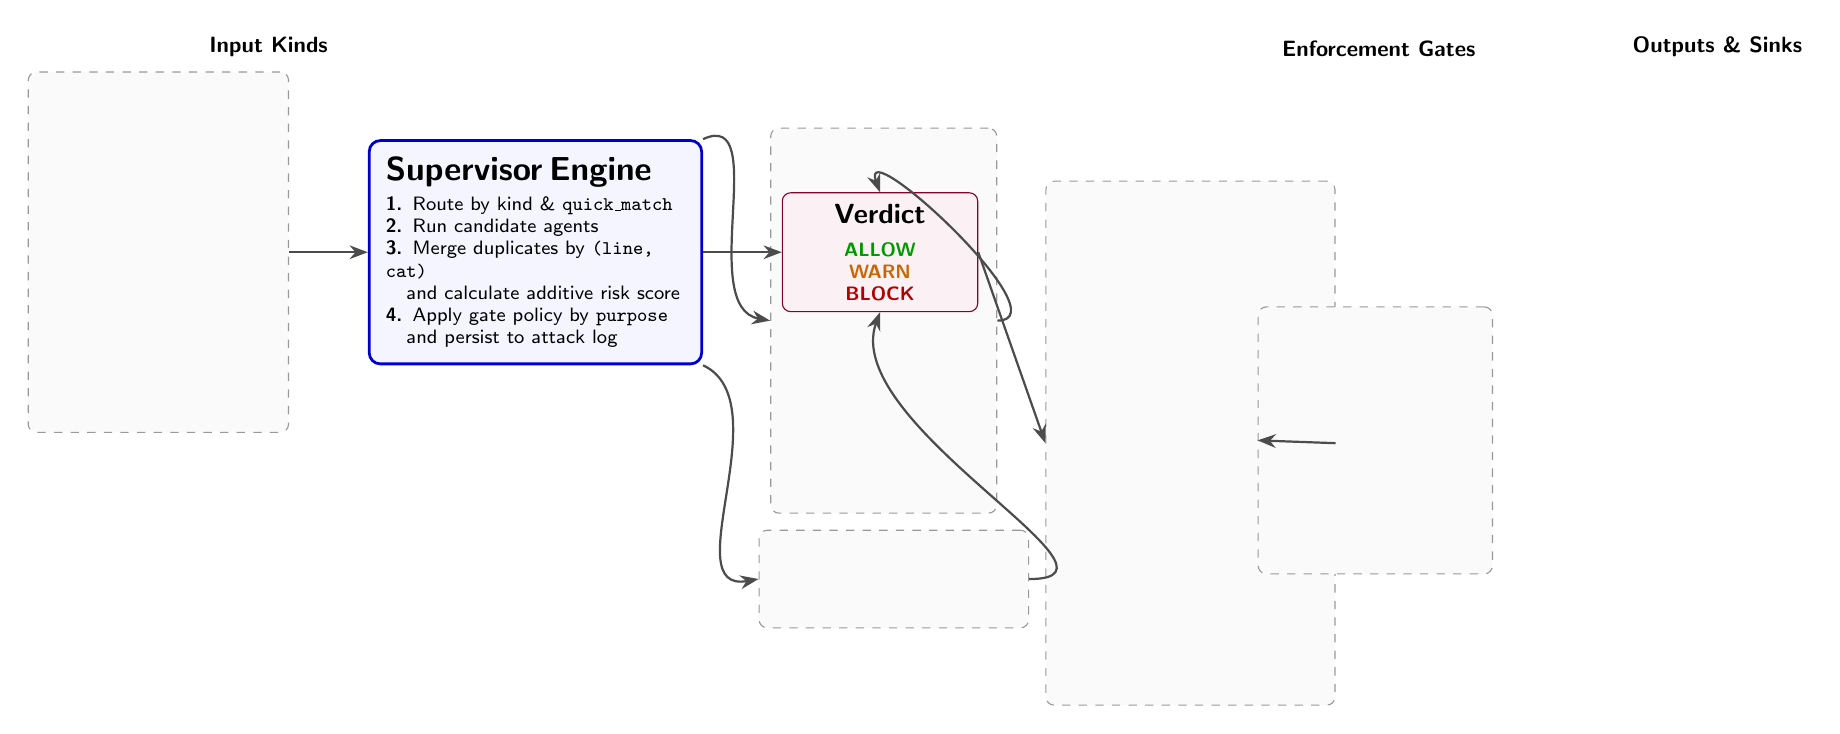
\begin{tikzpicture}[
    >=Stealth,
    font=\sffamily\small,
    kind/.style={draw=cyan!70!black, rounded corners=2pt, fill=cyan!8, inner sep=3pt, align=center, text width=2.8cm, font=\sffamily\scriptsize},
    supbox/.style={draw=blue!80!black, line width=1pt, rounded corners=4pt, fill=blue!4, inner sep=6pt, align=left, text width=3.8cm, font=\sffamily\scriptsize},
    agent-att/.style={draw=red!70!black, rounded corners=2pt, fill=red!6, inner sep=2.5pt, align=center, text width=2.4cm, font=\sffamily\scriptsize},
    agent-vuln/.style={draw=orange!80!black, rounded corners=2pt, fill=orange!8, inner sep=2.5pt, align=center, text width=2.4cm, font=\sffamily\scriptsize},
    verdict/.style={draw=purple!70!black, rounded corners=3pt, fill=purple!6, inner sep=4pt, align=center, text width=2.2cm, font=\sffamily\scriptsize},
    gate/.style={draw=teal!70!black, rounded corners=2pt, fill=teal!6, inner sep=2.5pt, align=center, text width=3.2cm, font=\sffamily\scriptsize},
    sink/.style={draw=blue!70!black, rounded corners=3pt, fill=blue!8, inner sep=4pt, align=center, text width=2.4cm, font=\sffamily\scriptsize},
    groupbox/.style={draw=black!40, dashed, rounded corners=3pt, inner sep=4pt, fill=black!2},
    arr/.style={->, line width=0.8pt, draw=black!70}
]

% 1. Input Kinds
\node[font=\sffamily\bfseries\footnotesize, anchor=south] at (1.4, 0.4) {Input Kinds};
\node[kind, at={(0,0)}] (kind0) {\texttt{USER\_SOURCE}};
\node[kind, below=0.18cm of kind0] (kind1) {\texttt{COMPILER\_OUTPUT}};
\node[kind, below=0.18cm of kind1] (kind2) {\texttt{AI\_RESPONSE}};
\node[kind, below=0.18cm of kind2] (kind3) {\texttt{USER\_HINT}};
\node[kind, below=0.18cm of kind3] (kind4) {\texttt{PATCH}};
\node[kind, below=0.18cm of kind4] (kind5) {\texttt{HTTP\_REQUEST}};
\node[kind, below=0.18cm of kind5] (kind6) {\texttt{MODEL\_FILE}};
\node[kind, below=0.18cm of kind6] (kind7) {\texttt{DATASET\_ENTRY}};
\node[groupbox, fit=(kind0) (kind7)] (kinds-group) {};

% 2. Supervisor Box
\node[supbox, right=1.0cm of kinds-group] (supervisor) {
    \textbf{\large Supervisor Engine}\\[3pt]
    \textbf{1.} Route by kind \& \texttt{quick\_match}\\
    \textbf{2.} Run candidate agents\\
    \textbf{3.} Merge duplicates by \texttt{(line, cat)}\\
    \quad and calculate additive risk score\\
    \textbf{4.} Apply gate policy by \texttt{purpose}\\
    \quad and persist to attack log
};

% 3. Agents in two groups
\node[font=\sffamily\bfseries\scriptsize, right=1.0cm of supervisor.north east, anchor=north west] (lbl-att) {Attacks on Tool};
\node[agent-att, below=0.2cm of lbl-att.south west, anchor=north west] (tagent0) {\texttt{ExecGuard}};
\node[agent-att, below=0.15cm of tagent0] (tagent1) {\texttt{ResourceGuard}};
\node[agent-att, below=0.15cm of tagent1] (tagent2) {\texttt{OutputGuard}};
\node[agent-att, below=0.15cm of tagent2] (tagent3) {\texttt{EndpointGuard}};
\node[agent-att, below=0.15cm of tagent3] (tagent4) {\texttt{SecretsGuard}};
\node[agent-att, below=0.15cm of tagent4] (tagent5) {\texttt{IntegrityGuard}};
\node[agent-att, below=0.15cm of tagent5] (tagent6) {\texttt{PromptGuard}};
\node[agent-att, below=0.15cm of tagent6] (tagent7) {\texttt{PatchGuard}};
\node[groupbox, fit=(lbl-att) (tagent0) (tagent7)] (tool-group) {};

\node[font=\sffamily\bfseries\scriptsize, below=0.35cm of tool-group.south west, anchor=north west] (lbl-vuln) {Weaknesses in User Code};
\node[agent-vuln, below=0.2cm of lbl-vuln.south west, anchor=north west] (uagent0) {\texttt{VulnGuard}};
\node[groupbox, fit=(lbl-vuln) (uagent0)] (user-group) {};

% 4. Verdict Box
\node[verdict, right=1.0cm of supervisor.east] (verdict-node) {
    \textbf{\normalsize Verdict}\\[4pt]
    \textcolor{green!60!black}{\textbf{ALLOW}}\\
    \textcolor{orange!80!black}{\textbf{WARN}}\\
    \textcolor{red!70!black}{\textbf{BLOCK}}
};

% 5. Enforcement Gates
\node[font=\sffamily\bfseries\footnotesize, anchor=south] at (15.5, 0.4) {Enforcement Gates};
\node[gate, right=1.0cm of verdict-node.north east, anchor=north west] (gate0) {\textbf{compile gate}\\\tiny{compiler\_runner, heal\_engine}};
\node[gate, below=0.16cm of gate0] (gate1) {\textbf{run gate}\\\tiny{gui.run\_code, web\_server}};
\node[gate, below=0.16cm of gate1] (gate2) {\textbf{AI-send gate}\\\tiny{ai\_explainer, ai\_healer, llm\_client}};
\node[gate, below=0.16cm of gate2] (gate3) {\textbf{patch gate}\\\tiny{ai\_healer}};
\node[gate, below=0.16cm of gate3] (gate4) {\textbf{request gate}\\\tiny{web\_server}};
\node[gate, below=0.16cm of gate4] (gate5) {\textbf{dataset gate}\\\tiny{dataset\_logger}};
\node[gate, below=0.16cm of gate5] (gate6) {\textbf{model-load gate}\\\tiny{ErrorClassifier}};
\node[gate, below=0.16cm of gate6] (gate7) {\textbf{display neutralisation}\\\tiny{output\_safe.safe\_text}};
\node[groupbox, fit=(gate0) (gate7)] (gates-group) {};

% 6. Outputs / Sinks
\node[font=\sffamily\bfseries\footnotesize, anchor=south] at (19.8, 0.4) {Outputs \& Sinks};
\node[sink, right=1.0cm of gates-group.center, anchor=west, yshift=1.2cm] (out0) {\textbf{Desktop GUI}\\\tiny{PyQt6 Student UI}};
\node[sink, below=0.4cm of out0] (out1) {\textbf{Web IDE}\\\tiny{Browser Interface}};
\node[sink, below=0.4cm of out1] (out2) {\textbf{Attack Log}\\\tiny{JSONL Security Record}};
\node[groupbox, fit=(out0) (out2)] (outs-group) {};

% Connective Arrows
\draw[arr] (kinds-group.east) -- (supervisor.west);
\draw[arr] (supervisor.east) -- (verdict-node.west);
\draw[arr] (supervisor.north east) to[out=25, in=170] (tool-group.west);
\draw[arr] (supervisor.south east) to[out=-25, in=190] (user-group.west);
\draw[arr] (tool-group.east) to[out=0, in=110] (verdict-node.north);
\draw[arr] (user-group.east) to[out=0, in=-110] (verdict-node.south);
\draw[arr] (verdict-node.east) -- (gates-group.west);
\draw[arr] (gates-group.east) -- (outs-group.west);

\end{tikzpicture}
\end{document}
